
\section{GAT-Denoiser}

\begin{frame}{GAT-Denoiser}
  \begin{itemize}
    \item GAT-Denoiser is a graph neural network (GNN) to denoise observations.
    \item Consists of three components:
    \begin{itemize}
      \item \alert<3-4>{Convolution}
      \only<4>{
        \begin{itemize}
          \item \alert{Denoise single observation}
        \end{itemize}
      }
      \item \alert<3-4>{Graph Attention Network (GAT) \cite{GAT}}
      \only<4>{
        \begin{itemize}
          \item \alert{Denoise neighboring  observation}
        \end{itemize}
      }
      
      \item \alert<5-6>{End-to-End Learning}
      \only<5-6>{
        \begin{itemize}
          \item<6> \alert{Optimize for reconstruction quality}
          \item<6> \alert{Loss: $\mathcal{L}_{reconstruction} = \parallel x - \textit{Recon} ( \textit{GAT-Denoiser}(y)) \parallel ^2_2$}
        \end{itemize}
      }
      
    \end{itemize}
  \end{itemize}
  

    \only<2>{
      \begin{figure}
        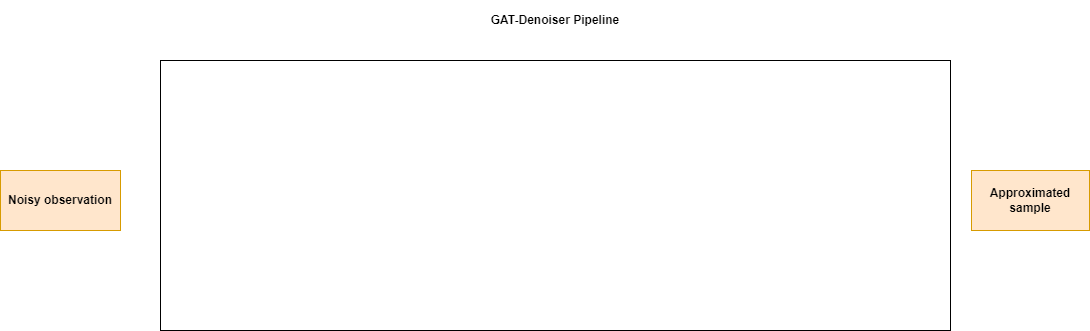
\includegraphics[width=.9\textwidth]{Overall_GAT-Denoiser_Pipeline_3.drawio.png}
      \end{figure}
    }

    \only<3-4>{
      \begin{figure}
        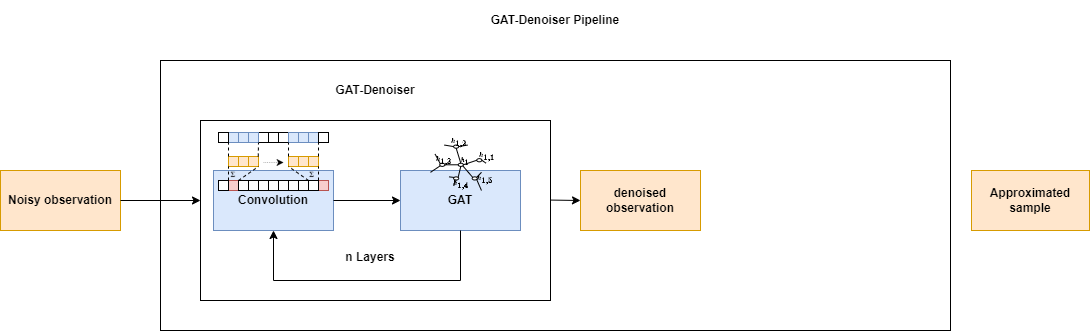
\includegraphics[width=.8\textwidth]{Overall_GAT-Denoiser_Pipeline_2.drawio.png}
      \end{figure}
    }

    \only<5-6>{
      \begin{figure}
        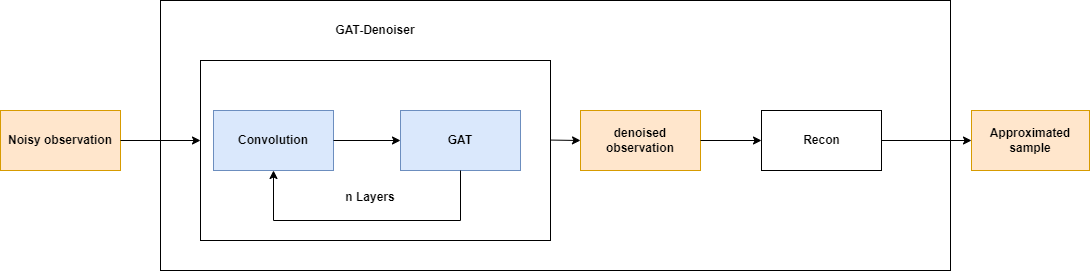
\includegraphics[width=.8\textwidth]{Overall_GAT-Denoiser_Pipeline.drawio.png}
      \end{figure}
    }

      
\end{frame}

% \begin{frame}{GAT-Denoiser Components}
    
%   \begin{itemize}
%     \item<2-> Convolution
%     \begin{itemize}
%       \item Denoise single observation
%     \end{itemize}

%     \item<3-> Graph Attention Network (GAT) \cite{GAT}
%     \begin{itemize}
%       \item Denoise neighboring  observation
%     \end{itemize}
%     \item<4-> End-to-End Learning
%     \begin{itemize}
%       \item Optimize for reconstruction quality
%       \item Loss: $\mathcal{L}_{reconstruction} = \parallel x - \textit{Recon} ( \textit{GAT-Denoiser}(y)) \parallel ^2_2$
      
%     \end{itemize}
%   \end{itemize}

% \end{frame}

\begin{frame}{Graph Attention Network - GAT}
  \pause
  \begin{columns}
  \column{0.6\textwidth}
    \begin{itemize}
      \item Extends Graph Convolution Network with attention (weights)
      \item Computes new node features
      \item Averages graph over neighborhood
      \item Multi-head available, motivated by \cite{transformer}
      \item<3> \alert<3>{$\sigma$: activation function (Exponential Linear Unit)}
      \item<3> \alert<3>{$W$: learnable weight matrix}
      \item<3> \alert<3>{$\alpha$: normalized attention coefficients}
    \end{itemize}
    \column{0.4\textwidth}
    \only<3>{
    \begin{figure}
      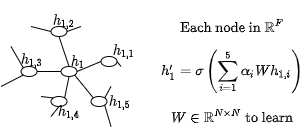
\includegraphics[width=.6\textwidth]{GAT.drawio.png}
    \end{figure}
      $$h_{1}^{\prime} = \sigma \left( \sum_{i=1}^6\alpha_i W h_{i} \right)$$
    }
    
  \end{columns}

\end{frame}


\begin{frame}{Input Graph}
  \pause
  \begin{columns}
    \column{0.6\textwidth}
    \begin{itemize}
      \item Exploit information from GL
      \begin{itemize}
        \item Low-dimensional embedding estimates angles
        \item Dominant information in data can be considered observation angles.
      \end{itemize}
      \item<3-> \alert<3>{Construct graph from observation angles}
      \begin{itemize}
        \item<4-> Map angles to unit-circle / unit-sphere
        \item<5-> Apply k-NN with great-circle distance
      \end{itemize}
    \end{itemize}
    \column{0.4\textwidth}

    \only<4>{
      \begin{figure}
        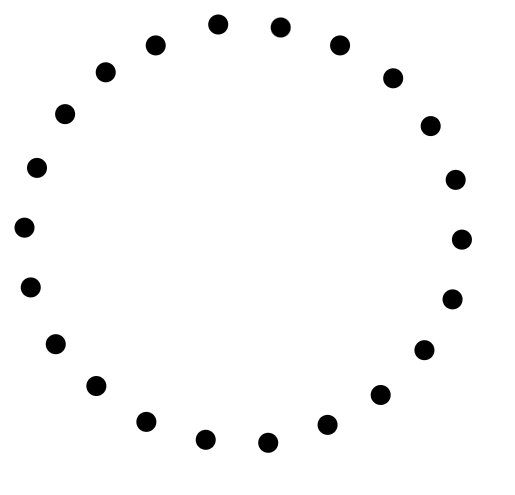
\includegraphics[width=.7\textwidth]{Circle_graph.drawio.png}
      \end{figure}
    }

    \only<5->{
      \begin{figure}
        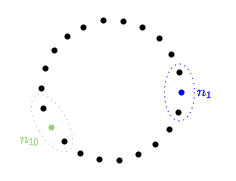
\includegraphics[width=.85\textwidth]{Circle_graphneighbours.drawio.png}
      \end{figure}
    }
    
  \end{columns}
  

  \begin{tcolorbox}[colback=red!5!white,hide=<1-5>, alert=<6>, colframe=red!75!black]
    Observation angles $\theta$ are assumed to be equally spaced on the unit-circle.
\end{tcolorbox}
\end{frame}

